\documentclass{article}
\usepackage[a4paper, margin=1in]{geometry} % Adjust margin size as needed
\usepackage{graphicx} % Required for inserting images
\usepackage{listings}
\lstset{basicstyle=\ttfamily}
\usepackage{float}
\usepackage{courier}
\usepackage{tabularx}
\usepackage{tikz}
\usepackage{url}
\usepackage{amsmath}
\usepackage{float}
\usepackage{hyperref}
\usepackage{MnSymbol}
\usepackage{indentfirst}

\title{Project: Report Document}
\author{Daniel Alejandro Marin - R11858881\\ \\ Texas Tech University \\CS3375 - Computer Architecture \\ Instructor: Dr. Juan Carlos Rojas}
\date{December 6$^{th}$, 2024}
\begin{document}
\maketitle
\tableofcontents
\newpage
\section{Introduction}
Instruction scheduling plays a crucial role in moder computer architecture, especially for achieving high performance in multi-issue processors; they allow for faster instruction throughput. This project aims to simulate the scheduling of `assembly' instructions under various processor configurations. The configurations developed in this project are the following:

\begin{itemize}
    \item Single-issue Instruction Scheduler (in-order)
    \item Superscalar Instruction Scheduler (in-order)
    \item Superscalar Instruction Scheduler (out of order) 
\end{itemize}

For each of this configurations there exists a version with register renaming and one without. In this project, we will simulate a the scheduling of a simple assembly instruction set, in each of these configurations. 

Throughout this report document, we will be explaining the design, implementation details, test and results of each configuration. The insights gained will highlight the advantages and limitations of these techniques in processor architectures. 

\section{Design and Methodology}
The instruction scheduling simulation system is designed as a hierarchy of classes that simulate different types of processor configurations for instruction fetching and retirement. The design uses abstraction and inheritance to encapsulate common functionality while allowing customization for specific scheduling techniques like: register renaming, in-order retirement, and out of order execution. Following is a class diagram that encapsulates the core design of this project.

\begin{figure}[H]
    \centering
    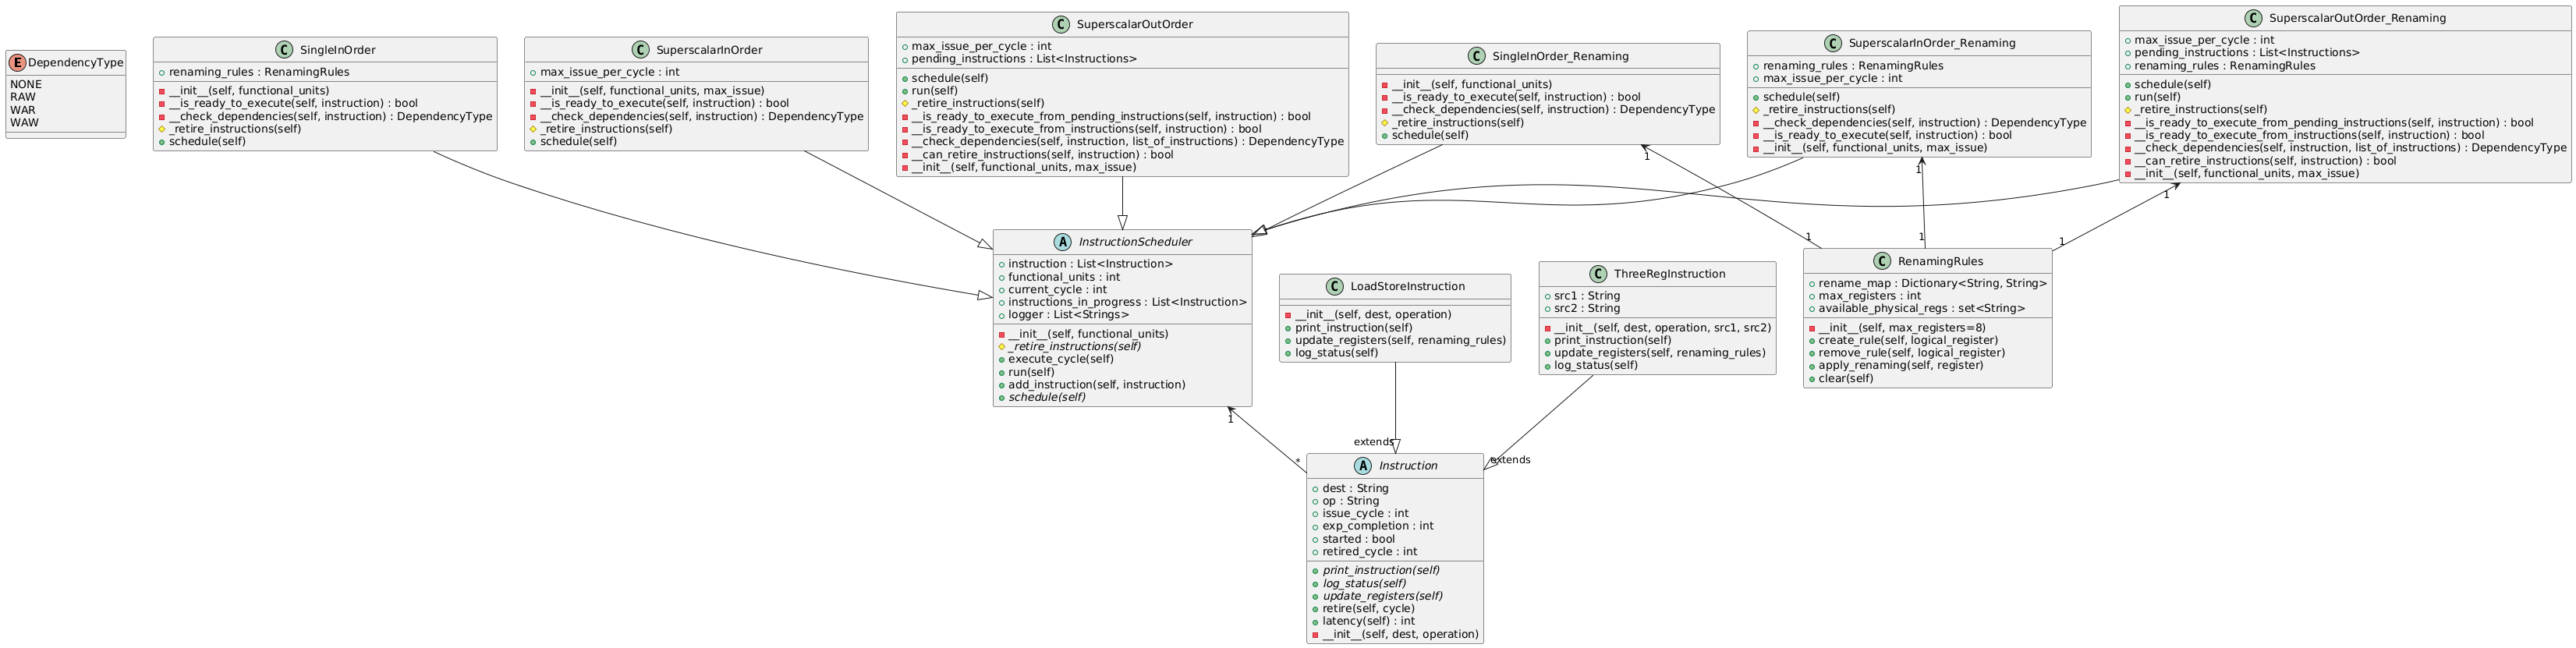
\includegraphics[width=1\textwidth]{ClassDiagram.png}  
    \caption{Class Diagram of Design, developed using the Plant UML tools.}  
    \label{fig:ClassDiagram}
\end{figure}

The diagram in figure \ref{fig:ClassDiagram} encapsulates the logic that helped develop this simulation. In the following subsections, I will be explaining each class with code snippets and implementation to justify each of the components. Before, delving into the overall classes let's discuss the format of the assembly instructions. 

\subsection{Assembly Format}
The assembly format contained various properties that where expected from the simulation, and some that I saw fit. It can be explained with the following:

\begin{itemize}
    \item There are 8 fixed registers (R0 to R7) used in the assembly code
    \item There are only 5 instruction operations: +, -, *, LOAD, and STORE
    \item The format of the instructions are as follow: R1 = LOAD, R2 = STORE, R0 = R1 + R7, R1 = R2 * R3, etc\ldots
    \item +, - instructions take 1 cycle to complete
    \item * take 2 cycles to complete 
    \item LOAD, STORE take 3 cycles to complete
\end{itemize}

This assembly format ended up being used to develop the tests used to demonstrate proper functionality when simulating. The classes in charge of containing the instructions that derive from the assembly are the ones that compose the instruction hierarchy.

\subsection{Instruction Hierarchy}
The Instruction Hierarchy is used to encompass methods and data that provide access to the instructions as individual components when simulating, containing properties such as: source registers, destination registers, etc\ldots The parent class of this hierarchy is the \lstinline|Instruction| abstract class which contained the following properties:

\begin{itemize}
    \item \lstinline|dest|: this property looked to contain the destination register of an instruction. Allowing easy access to this information when required by the instruction schedulers.
    \item \lstinline|op|: this one contained the type of operation that the current instance is supposed to hold, determining the latency for further properties.
    \item \lstinline|issue_cycle|: this integer contained the processor cycle in which the instance of the instruction was issued.
    \item \lstinline|exp_completion|: this property contained the expected completion cycle for an instruction, stating after which point the instruction could be retired. 
    \item \lstinline|started|: this is a boolean that was raised when the instruction was issued, implying that I have (in a sense) been scheduled. 
    \item \lstinline|retired_cycle|: this property contained the actual cycle in which the instruction got retired by the processor configuration.
\end{itemize}

These properties where present in all types of instructions defined in the assembly format, the only work around done was that for `STORE' instructions filled the `destination register' with it's source register. Thus, leading to certain checks when handling dependencies.

The methods in this class, where used to extract information from the instructions themselves, so that the code would be less repeated. 

\begin{itemize}
    \item \lstinline|print_instruction(self)|: abstract method in charge of printing instructions. This is used to print out each instruction in the command line.
    \item \lstinline|log_status(self)|: abstract method in charge of logging the status of the instruction at given points of the scheduling. This method logs the issue cycle and the retire cycle when called. Used for debugging and printing.
    \item \lstinline|update_registers(self, renaming_rules)|: abstract method in charge of updating the source registers that compose an instruction based on the renaming rules, basically applying renaming rules.
    \item \lstinline|retire(self, cycle)|: method in charge of retiring an instruction when called. Used when an instruction has been completely scheduled, exited the pipeline.
    \item \lstinline|latency(self)|: method in charge of retrieving the latency of any instruction, used for calculating some of the properties.
\end{itemize}

This abstract class does not represent instructions as a whole. Instead they represent a base for the concrete types of instructions that inherit from them. The concrete classes that inherit from \lstinline|Instruction| are \lstinline|LoadStoreInstruction| and \lstinline|ThreeRegInstruction|.
\subsubsection{Three Register Instructions}
The \lstinline|ThreeRegInstruction| class contains two more properties: \lstinline|src1| and \lstinline|src2|; and defines the abstract methods with their desired behavior. These properties combined with the properties from the parent class \lstinline|Instruction| allow an instance to represent a Three Register Instruction such as: R1 = R2 + R3.

\subsubsection{Load and Store Instructions}
The \lstinline|LoadStoreInstruction| only defines the abstract methods from \lstinline|Instruction| allowing an instance of itself to represent a Load or a Store Instruction such as: R1 = STORE. Now that we understand the representation of instructions we may begin looking at how register renaming rules where implemented. 

\subsection{Register Renaming Rules}
Register renaming rules where implemented with a class that was a part of any processor configuration that contained the technique. The class was named \lstinline|RenamingRules| and it contained properties and methods in charge of handling, applying and removing renaming rules as the scheduling of a set of instructions took place. The properties it contained where as follows:

\begin{itemize}
    \item \lstinline|rename_map|: this essentially a dictionary that relates a register from assembly (logical register) to a hidden register (physical register), like a rule relating the two. 
    \item \lstinline|max_registers|: the maximum number of registers, this represents the physical registers that where used when applying the register renaming technique. Represented by registers such as: S0, S7, etc.
    \item \lstinline|available_physical_registers|: represent the remaning number of registers available for renaming based on the number of renaming rules currently in place. 
\end{itemize}

The properties in this class are used to represent renaming rules in the program, yet to create new rules and delete invalid rules, I created two methods in charge of this. Those methods are:

\begin{itemize}
    \item \lstinline|create_rule(self, logical_register)|: this method creates a rule for the logical register it receives (e.g: \lstinline|R0 => S1|). The code in charge of doing this is fairly simple. 
\begin{lstlisting}[language=Python]
    def create_rule(self, logical_register):
        if logical_register not in self.rename_map:
            if not self.available_physical_regs:
                return False 
            physical_register = self.available_physical_regs.pop() 
            self.rename_map[logical_register] = physical_register
            return True
        return False
\end{lstlisting}
    This snippet of the program creates a mapping between one of the available hidden registers and the register it received as input. 
    \item \lstinline|remove_rule(self, logical_register)|: this method is in charge of removing rules for a certain logical register, it looks to invalidate existing renaming rules. The function is as follows:
\begin{lstlisting}
        if logical_register in self.rename_map:
            physical_register = self.rename_map.pop(logical_register)
            self.available_physical_regs.add(physical_register) 
            return True
        return False
\end{lstlisting}
    Essentially, it removes the mapping between the logical register and the hidden register; and returns the hidden register to an available state. 
\end{itemize}

The use of the properties and methods in \lstinline|RenamingRules| in coordination with the processor scheduling configuration leads the technique of register renaming to be properly simulated in this program. Now, let's delve into the instruction schedulers.

\subsection{Instruction Scheduler Hierarchy}
The Instruction Scheduler Hierarchy is the family of classes that contain the main logic of the scheduling simulation. The parent class of this hierarchy is \lstinline|InstructionScheduler| class which contains a layout of properties and methods to develop each configuration. All other classes that persist above it are the concrete classes.

This section looks to encompass the most important concepts that simulate the desired behavior of each configuration. To understand this we won't look at individual classes but more at what overlapping techniques, properties and functions look like, and look to explain what each part looks to provide to a scheduler class.  This is done, because each configuration (set of capabilities) is a selection of these components. 

Let's begin by looking at the list of all the properties that the classes in this hierarchy contain, explaining what they provide and which classes contain them.

\begin{itemize}
    \item \lstinline|instructions|: a list of instructions that need to be scheduled by the current configuration. \textbf{All configurations} contain this. 
    \item \lstinline|functional_units|: the number of parallel functional units a process configuration has. \textbf{All configurations} contain this.
    \item \lstinline|current_cycle|: contains the current cycle being executed by the processor. \textbf{All configurations} contain this.
    \item \lstinline|instructions_in_progress|: contains the list of instructions that are in functional units, currently being executed. \textbf{All configurations} contain this.
    \item \lstinline|logger|: contains a list of strings that represent debug messages and statements of actions that are taking place while scheduling. \textbf{All configurations} contain this, and it represents a list of outputs.
    \item \lstinline|max_issue_per_cycle|: the number of issue slots per cycle for a certain configuration. Only \textbf{Superscalar configurations} contain this property, because it represents it indicates how many instructions should be attempted per executed cycle.
    \item \lstinline|pending_instructions|: a list of instructions that have been overlooked/skipped by the processor configuration. This list is only present in \textbf{configurations with Out of Order execution}.
    \item \lstinline|renaming_rules|: contains an instance of the \lstinline|RenamingRules| class to create, delete and map renaming rules. This instance is only present in configurations that apply the \textbf{register renaming technique}. 
\end{itemize}

\subsection{Instruction Scheduler Abstract Class}
The \lstinline|InstructionScheduler| abstract class defined the layout all configurations of instructions schedulers should follow. It defined the main components and methods they should have, and contained some of the overlapping logic that remained consistent throughout all configurations. It contained the following properties:
\begin{itemize}
    \item \lstinline|instructions|: this property looks to contain a list of instructions that need to be scheduled in the simulation.
    \item \lstinline|functional_units|: this property represents the number of parallel functional units the scheduler has. It is a property defined by the user. 
    \item \lstinline|current_cycle|: this property contains the current cycle of execution of the processor.
    \item \lstinline|instructions_in_progress|: this property contains the list of instructions that are currently being executed. 
    \item \lstinline|logger|: this property contains a `log book' of the logs performed by the scheduler, used for debug statements and keeping track of instructions in the order they retire (outputs).
\end{itemize}

These are the properties all schedulers contained, additional properties can be added to the subclasses of \lstinline|InstructionScheduler| when needed. Now, let's look at the methods defined in this parent class in the following itemize:
\begin{itemize}
    \item \lstinline|__init__(self, functional_units=1)|: this constructor method is used to create instances of this class, and it is called by the children classes as to initialize the aforementioned properties. 
    \item \lstinline|add_instruction(self, instruction)|: this method is in charge of adding an instruction to \lstinline|instructions|. It is used to add parsed instructions set that we want to simulate the scheduling.
    \item \lstinline|execute_cycle(self)|: this method contains the logic of executing a cycle in the simulation incrementing \lstinline|current_cycle| by one, attempting to schedule instructions, and retiring instructions. The definition is as follows:
    \begin{lstlisting}
    def execute_cycle(self):
        self.current_cycle += 1
        self.schedule()
        self._retire_instructions()
    \end{lstlisting}
    \item \lstinline|run(self)|: this method is fairly straightforward, it executes cycles until all instructions have been dispatched out of the scheduler. Most configurations used the definition:
    \begin{lstlisting}{language=Python}
    def run(self):
        while self.instructions or self.instructions_in_progress:
            self.execute_cycle()
    \end{lstlisting}
    \item \lstinline|schedule(self)|: this method contains the logic for scheduling instructions. It is abstract, since each subclass configuration schedules instructions differently. 
    \item \lstinline|_schedule_instruction(self, instr : Instruction)|: this method is in charge of updating the status of an instruction whenever it gets scheduled. It does so in the following manner:
    \begin{lstlisting}{language=Python}
    def _schedule_instruction(self, instr : Instruction):
        instr.issue_cycle = self.current_cycle
        instr.exp_completion = self.current_cycle + instr.latency()
        instr.started = True 
        self.instructions_in_progress.append(instr)
    \end{lstlisting}
    \item \lstinline{_retire_instructions(self)}: this method should contains the logic for retiring instructions. It is abstract, since each subclass configuration retires instructions differently.
\end{itemize}

\subsection{Instruction Scheduler's}
In this section we will be discussing the various concrete classes that make up the actual instruction scheduler's. Before looking at each configuration individually let's look at all the version's / processor capabilities developed:
\begin{itemize}
    \item Single instruction, in-order execution
    \item Superscalar, in-order execution
    \item 
\end{itemize}

\section{Methodology}

\section{Tests}

\section{Results}

\section{Discussion}

\end{document}